
\section*{Slides additionnels}

\begin{frame}{Document}{Spécification}
  \begin{definition}[Spécification séquentielle d'une séquence]
  Soit une série d'opérations $H$ produisant la séquence
  $s(H) = \{p_1,\, p_2 \ldots p_k\}$ avec $p_{1..k} \in \mathcal{P}$ où
  $\mathcal{P}$ est un ensemble muni d'un ordre
  dense $(\mathcal{P},\,<_\mathcal{P})$ tel que : \\
  $\forall p\in\mathcal{P},\, p_\vdash <_\mathcal{P} p <_\mathcal{P} p_\dashv $
  \hfill et \ \
  $p_\vdash <_\mathcal{P} p_1 <_\mathcal{P} p_2 <_\mathcal{P} \ldots
  <_\mathcal{P} p_k <_\mathcal{P} p_\dashv$.
  
  \vspace{0.25cm}

  \noindent L'insertion d'un élément $e$ en position $i$ dans la séquence $s(H)$
  est définie de la façon suivante :
  \begin{equation}
    \small
    s(H \cup INSERT(i,\, e)) \rightarrow s(H) \cup 
    \begin{cases}
      \{p,\, p_\vdash <_\mathcal{P} p <_\mathcal{P} p_\dashv \} & i = 0 \wedge |s(H)| = 0\\
      \{p,\, p_\vdash <_\mathcal{P} p <_\mathcal{P} p_1 \} & i = 0 \wedge |s(H)|>0\\
      \{p,\, p_k <_\mathcal{P} p <_\mathcal{P} p_\dashv \} & i = k\\
      \{p,\, p_i <_\mathcal{P} p <_\mathcal{P} p_{i+1} \} & sinon
    \end{cases}
  \end{equation}

  \noindent La suppression de l'élément en position $i$ dans la séquence $s(H)$
  est définie de la façon suivante :
  \begin{equation}
    \small
    s(H \cup DELETE(i)) \rightarrow s(H) \setminus \{ p_i \}
  \end{equation}
\end{definition}
\end{frame}


\begin{frame}{Document}{Complexité temporelle des accès}
  
  \begin{center}
    
\small
\begin{tabularx}{0.7\textwidth}{@{}Xc@{}}
  \toprule
  \textsc{Comportement d'édition} & \textsc{Temps} \\
  & \ \ \ \ \ \ \ \ \ \textsc{lookup} \ \ \ \ \ \ \ \ \ \\ \midrule
  Édition aléatoire & $\mathcal{O}(2^{\sqrt{\log I}})$ \\
  Édition monotone / pire cas & $\mathcal{O}(I)$ \\ \bottomrule
%%  Worst case & $\mathcal{O}(I)$ \\ \bottomrule
\end{tabularx}


  \end{center}
  
  \vspace{0.25cm}%
  \begin{center}%
  \begin{tikzpicture}[scale=0.9]
  \newcommand\X{30pt}
  \newcommand\Y{45pt}

  \small
  \draw[dashed, thick] (0pt,0pt) -- node[anchor=south east]{0} (-3.5*\X,-1*\Y);
  \draw[thick, color=darkblue] (0pt,0pt) --
  node[anchor=west]{\DARKBLUE{1}} (-2.5*\X,-1*\Y);
  \draw[thick] (-2.5*\X,-1*\Y) -- node[anchor=east]{3} (-1.5*\X,-2*\Y);
  \draw[thick] (-2.5*\X,-1*\Y) -- node[anchor=east]{7} (-0.5*\X, -2*\Y);
  \draw[thick] (-2.5*\X,-1*\Y) -- node[anchor=west]{11} (0.5*\X,-2*\Y);
  \draw[thick, color=darkblue](0pt,0pt) -- 
  node[anchor=west]{\DARKBLUE{5}} ( 1.5*\X,-1*\Y);
  \draw[thick, color=darkblue] (1.5*\X,-1*\Y) -- 
  node[anchor=west]{\DARKBLUE{4}} (2.5*\X,-2*\Y);
  \draw[dashed, thick] (0pt,0pt) -- node[anchor=south west]{8} ( 3.5*\X,-1*\Y);

  \draw[->, color=darkblue] (-2.5*\X,-1*\Y) -- (-2.5*\X,-10-1*\Y);
  \draw[->] (-1.5*\X,-2*\Y) -- (-1.5*\X,-10-2*\Y);
  \draw[->] (-0.5*\X,-2*\Y) -- (-0.5*\X,-10-2*\Y);
  \draw[->] ( 0.5*\X,-2*\Y) -- ( 0.5*\X,-10-2*\Y);
  \draw[->, color=darkblue] ( 1.5*\X,-1*\Y) -- ( 1.5*\X,-10-1*\Y);
  \draw[->, color=darkblue] ( 2.5*\X,-2*\Y) -- ( 2.5*\X,-10-2*\Y);

  \draw[fill=white, draw=darkblue](-2.5*\X,-14-1*\Y)
  node{\DARKBLUE{\textbf{Q}}}+(-4pt,-4pt)rectangle+(4pt,4pt);
  \draw[fill=white](-1.5*\X,-14-2*\Y)node{\textbf{W}}+(-4pt,-4pt)rectangle+(4pt,4pt);
  \draw[fill=white](-0.5*\X,-14-2*\Y)node{\textbf{E}}+(-4pt,-4pt)rectangle+(4pt,4pt);
  \draw[fill=white]( 0.5*\X,-14-2*\Y)node{\textbf{R}}+(-4pt,-4pt)rectangle+(4pt,4pt);
  \draw[fill=white, draw=darkblue]( 1.5*\X,-14-1*\Y)
  node{\DARKBLUE{\textbf{T}}}+(-4pt,-4pt)rectangle+(4pt,4pt);
  \draw[fill=white, draw=darkblue]( 2.5*\X,-14-2*\Y)
  node{\DARKBLUE{\textbf{Y}}}+(-4pt,-4pt)rectangle+(4pt,4pt);

  \draw[fill=darkblue] (  0pt,  0pt) circle (1pt);
  \draw[fill=black] (-3.5*\X,-1*\Y) circle (1pt);
  \draw[fill=white, draw=darkblue] (-2.5*\X,-1*\Y) circle (1pt);
  \draw[fill=white] (-1.5*\X,-2*\Y) circle (1pt);
  \draw[fill=white] (-0.5*\X,-2*\Y) circle (1pt);
  \draw[fill=white] ( 0.5*\X,-2*\Y) circle (1pt);
  \draw[fill=white, draw=darkblue] ( 1.5*\X,-1*\Y) circle (1pt);
  \draw[fill=white, draw=darkblue] ( 2.5*\X,-2*\Y) circle (1pt);
  \draw[fill=black] ( 3.5*\X,-1*\Y) circle (1pt);

  \draw[->, very thick, densely dashdotted] (15-2.5*\X,-1*\Y) --
  node[anchor=south]{\textbf{explore}} (-20+1.5*\X, -1*\Y) -- (-20+2.5*\X, -2*\Y);


\end{tikzpicture}
  \end{center}%
  
\end{frame}


\begin{frame}{Document}{Effets de la concurrence}
  \vspace{-0.5cm}
  \begin{center}
    \includegraphics[angle=-90, width=\textwidth]{img/replication/latency.eps}
  \end{center}
\end{frame}


\begin{frame}{Document}{Traces réelles}
  
  \hspace{-1cm}
  \begin{minipage}{0.45\textwidth}
    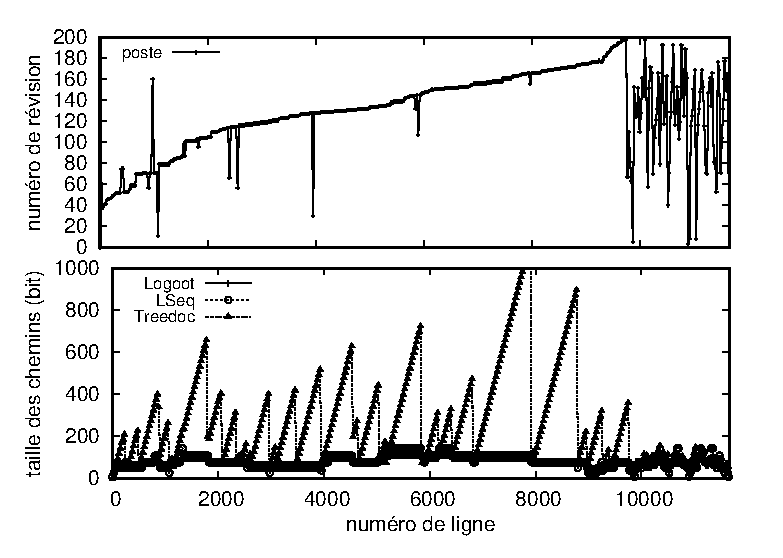
\includegraphics[width=1.29\textwidth]{img/replication/poste.eps}
  \end{minipage}
  \hspace{1.2cm}
  \begin{minipage}{0.45\textwidth}
      {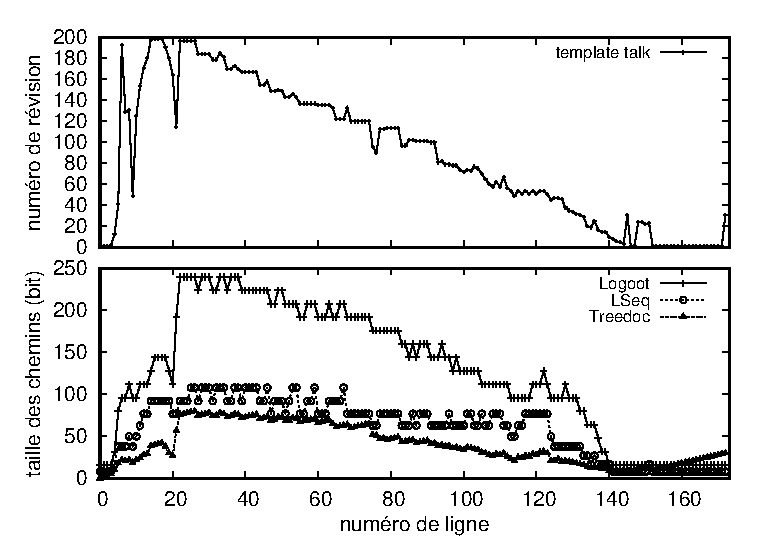
\includegraphics[width=1.29\textwidth]{img/replication/templatetalk.eps}}
  \end{minipage}

  \begin{minipage}{0.4\textwidth}
    Document édité en fin
  \end{minipage}
  \hspace{1.6cm}
  \begin{minipage}{0.4\textwidth}
      {Document édité au début}
  \end{minipage}

\end{frame}


\begin{frame}{Communication}{Échec de connexion}

  \begin{center}
    \begin{tikzpicture}[scale=1.]

\newcommand\X{40pt}
\newcommand\Y{-40pt}

  \draw (-\X, 0); %% align texts

  \small
  \draw (0pt,5pt)node[align=left,anchor=south]{$1_{initie}$\\
    $3_{ach\grave{e}ve}$};
  \draw (2*\X, 5pt)node[anchor=south east]{$2_{accepte}^{Cyclon}$};
  \draw(4*\X,5pt)node[anchor=south]{$2_{accepte}^{Scamp}$};
  \draw (3.5*\X, 0.5*\Y)node{\DARKBLUE{\ldots}};

  \draw[dashed](2*\X,-5pt)--(2*\X,-5+1*\Y);
  \draw[dashed](2*\X, 5pt)--(2*\X, 20pt);

  \normalsize
  \draw[fill=white, thick, draw=darkblue] (0pt, 0pt)
  node{\DARKBLUE{$n_1$}} +(-5pt,-5pt) rectangle +(5pt,5pt);
  \draw[fill=white] (1*\X,\Y) node{$n_2$} +(-5pt,-5pt) rectangle +(5pt,5pt);
  \draw[fill=white] (2*\X, 0pt) node{$n_3$} +(-5pt,-5pt) rectangle +(5pt,5pt);
  \draw[fill=white] (3*\X,\Y) node{$n_4$} +(-5pt,-5pt) rectangle +(5pt,5pt);
  \draw[fill=white, thick, draw=darkblue] (4*\X, 0pt) node{\DARKBLUE{$n_k$}}
  +(-5pt,-5pt) rectangle +(5pt,5pt);


  \draw[->] ( 0pt,-5pt) to[out=-85,in=175] (-5+1*\X,\Y);
  \draw[->, densely dashed] (1*\X, 5+\Y) to[out=95,in=-5] ( 5pt, 0pt);
  \draw     ( 5+1*\X, \Y) to[out=5,in=-95] (2*\X,-5pt);
  \draw[densely dashed] ( -5+2*\X, 0pt) to[out=185,in=85] (1*\X, 5+\Y);
  \draw[->] (2*\X, -5pt) to[out=-85,in=175] (-5+3*\X, \Y);
  \draw[->, densely dashed] (3*\X, 5+\Y) to[out=95,in=-5] (5+2*\X,0pt);
  \draw[->] (5+3*\X, \Y) to[out=5pt,in=-95] (4*\X,-5pt);
  \draw[densely dashed] (-5+4*\X, 0pt) to[out=185,in=85] (3*\X, 5+\Y);
%%  \draw[->, densely dashed] (-70pt, 0pt) -- (-30pt, 0pt); %% u1 -> u4
%%  \draw[->, densely dashed] (-5pt, 30pt) -- (-70pt, 5pt); %% u3 -> u1
%%  \draw[->, densely dashed] (30pt, -5pt) to[out=-85,in=-95](-70pt,-5pt);%%u5 u1

  \small 
  \begin{scope}[shift={(4.5*\X,0pt)}]
    \draw[->](0pt, -12pt)--(10pt, -12pt) node[anchor=west]{Aller};
    \draw[->, densely dashed](0pt, -19pt)--(10pt, -19pt)
    node[anchor=west]{Retour};    
  \end{scope}
  
\end{tikzpicture}
  \end{center}

  \vspace{1cm}

  \begin{equation} P_{E}^{Scamp}=1-(1- P_f)^{k+1} \end{equation}

  \vspace{0.5cm}

  \begin{align} P_{E,\,webrtc}^{Scamp} &=1 - ((1-P_f)^{2(k+1)} (1-P_f)^{2k}
                                         \ldots (1-P_f)^2) \nonumber \\
                                       &=1-(1-P_f)^{k^2+3k+2}
  \end{align}
  
\end{frame}

\begin{frame}{Communication}{L'information se propage rapidement}
  \begin{center}
    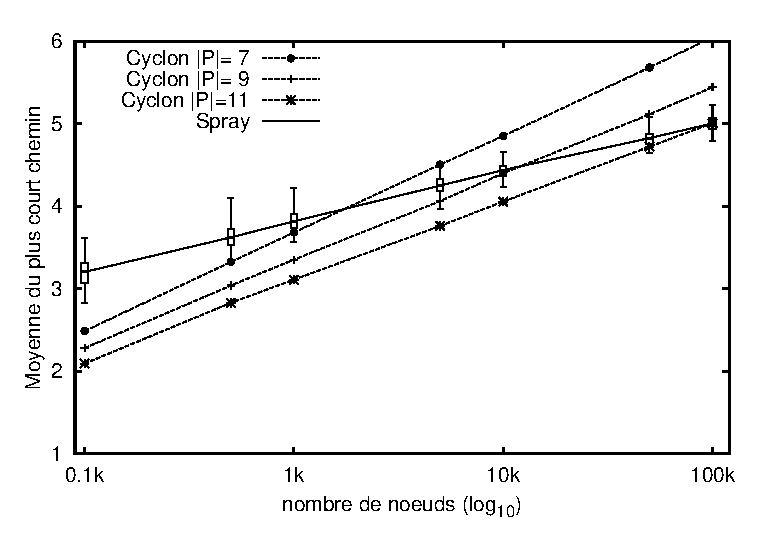
\includegraphics[width=1\textwidth]{img/network/avgpath.eps}
  \end{center}
\end{frame}

\begin{frame}{Communication}{La charge est équilibrée}
  \begin{center}
    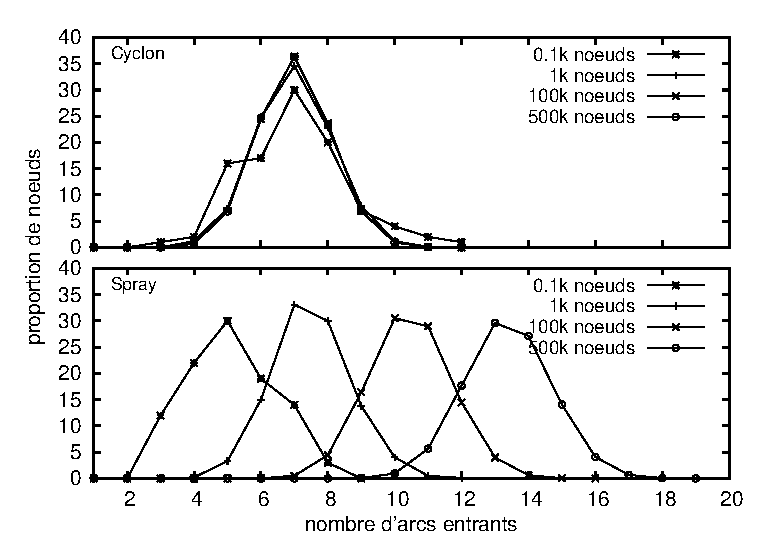
\includegraphics[width=1\textwidth]{img/network/histo.eps}
  \end{center}
\end{frame}

\begin{frame}{Communication}{Robuste aux défaillances}
  \begin{center}
    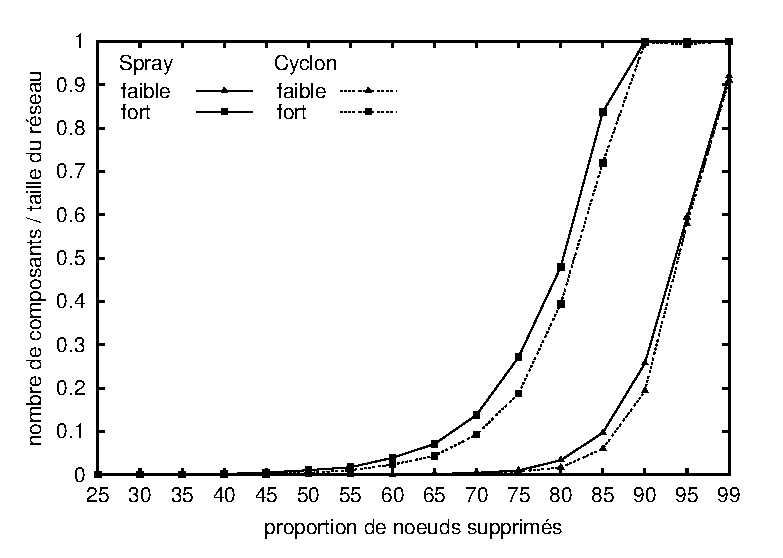
\includegraphics[width=1\textwidth]{img/network/resilience.eps}
  \end{center}
\end{frame}
